\chapter{Results and Discussion}\label{ch:results}
\section{Evidence scope}
This chapter uses the existing complete five-initialization experiments on five fixed graphs and four configurations. All 100 saved final evaluations were checked against their Spread, Coverage, and CELF scalars. Every cell contains exactly seeds 0--4. The results remain development evidence, with no claim of independent confirmation or selection of favorable runs \cite{projectdev}.

\section{Coverage across the four configurations}
\begin{table}[htbp]
\centering\small
\caption{Coverage mean $\pm$ sample SD (\%): all five fixed initialization seeds 0--4 per graph and configuration ($n=5$ per cell; 100 runs total). Existing development evidence; no seed selection.}\label{tab:coverage}
\begin{tabular}{lrrrr}
\toprule
Graph & Non-Private & Uniform1 & PDP v2 & Uniform4\\ \midrule
Email & 92.083 $\pm$ 2.099 & 82.130 $\pm$ 11.156 & 86.759 $\pm$ 10.791 & 89.259 $\pm$ 6.829 \\
Bitcoin & 98.694 $\pm$ 0.931 & 73.599 $\pm$ 25.250 & 81.971 $\pm$ 27.105 & 97.969 $\pm$ 0.731 \\
LastFM & 95.114 $\pm$ 1.268 & 77.289 $\pm$ 20.434 & 76.564 $\pm$ 32.386 & 91.206 $\pm$ 8.907 \\
HepPh & 81.493 $\pm$ 1.925 & 84.136 $\pm$ 9.168 & 80.563 $\pm$ 13.719 & 83.079 $\pm$ 13.375 \\
Facebook & 92.461 $\pm$ 2.277 & 87.608 $\pm$ 11.977 & 73.405 $\pm$ 29.099 & 74.539 $\pm$ 24.121 \\
\bottomrule\end{tabular}
\end{table}

Table~\ref{tab:coverage} reports the arithmetic mean and sample SD of five individual fits per cell. These are descriptive statistics, not proof that one method has higher population utility or lower variance. Non-Private is more concentrated in these five-seed records, but several training operations differ, so it does not isolate one source of instability.

Private results can vary substantially within the same cell. LastFM PDP v2 has Coverage values 80.693, 91.726, 19.701, 93.223, and 97.478\%, giving $76.564\pm32.386$\%. Four relatively high outcomes coexist with one severe loss; retaining that loss produces the large SD. It is not a formatting error or a repeated-evaluation artifact. All seeds are shown in Appendix~\ref{app:development}.

\begin{figure}[htbp]
\centering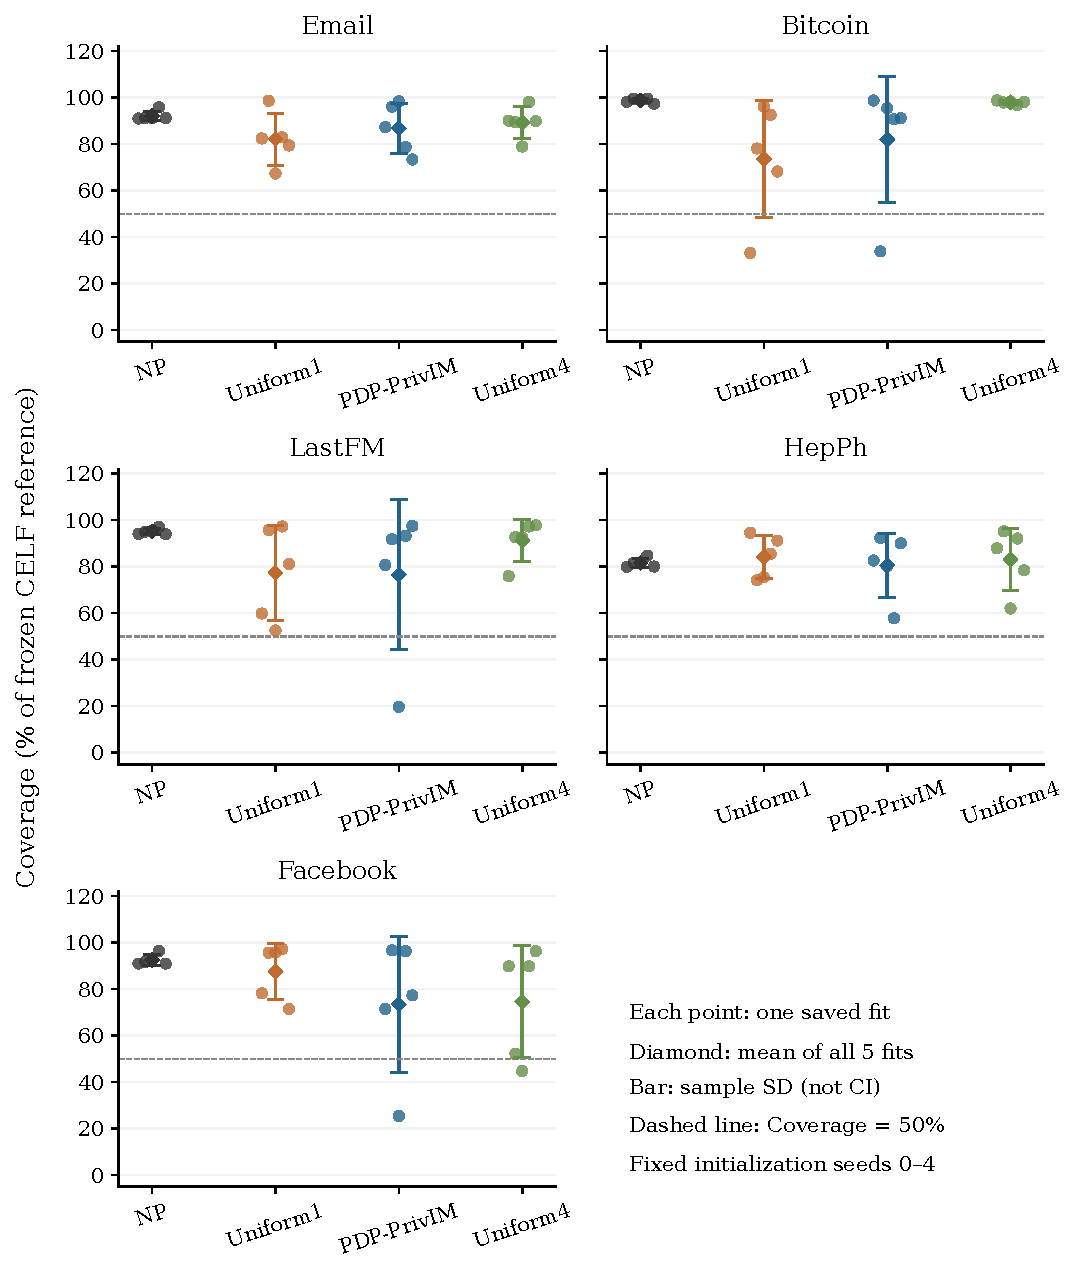
\includegraphics[width=.96\textwidth]{figures/five_seed_coverage.pdf}
\caption{All five Coverage outcomes per configuration and graph. Points are individual fits; diamonds and bars show mean and sample SD, not confidence intervals. Horizontal offsets only separate points visually. Every saved outcome is included.}\label{fig:fiveseed}
\end{figure}

Uniform4 has sample SD 0.731 pp on Bitcoin but 24.121 pp on Facebook under the same nominal noise scale. Its Facebook values include a severe low outcome. Uniform1 and PDP also show different responses across graphs. Such heterogeneity does not identify graph size or any particular topology statistic as the cause; the graphs differ in many uncontrolled ways.

\section{Verified update scales and bounded signal}
The common private kernel first clips each subgraph gradient, then clips each slot sum to norm at most 3. With four slots, the combined signal $S_t$ satisfies $\|S_t\|_2\leq12$. The pre-projection update is
\begin{equation}
 \Delta\theta_t=-\frac{0.005}{16}(S_t+Z_t),\qquad
 Z_t\sim\mathcal N(0,\sigma^2I_{2340}).
\end{equation}
Therefore the signal update has norm at most 0.00375. The Gaussian increment has coordinate SD $0.005\sigma/16$ and root mean square Euclidean norm $\sqrt{2340}\,0.005\sigma/16$.

\begin{table}[htbp]
\centering\small
\caption{Verified pre-projection update scales from frozen public constants. RMS means $\sqrt{\mathbb E\|\Delta\theta_{\rm noise}\|_2^2}$; it is not a Coverage SD or a measured gradient SNR.}\label{tab:noisescale}
\begin{tabular}{lrrr}\toprule
Configuration & Coordinate noise SD & Noise L2 RMS & Signal norm bound\\\midrule
Uniform1 & 0.151875 & 7.346732 & 0.003750\\
PDP v2 & 0.081250 & 3.930351 & 0.003750\\
Uniform4 & 0.043438 & 2.101226 & 0.003750\\\bottomrule
\end{tabular}
\end{table}

These scales make noise-driven parameter trajectories a well-motivated concern: full-coordinate random increments are large relative to the bounded signal. However, the signal bound is an upper bound rather than an observed useful gradient, and parameters can have redundant functional directions. The numbers do not identify a fraction of Coverage variance, establish a function-space SNR, or describe the final distribution after adaptive gradients and projection. Multiplying by $\sqrt{100}$ would describe only an additive independent-noise reference, not the actual trained model.

\section{Historical controlled evidence for Gaussian-path sensitivity}
A separate historical G2 diagnostic held initialization, the retained graph, slot caches, and all 100 batches fixed within each of 12 pairs, while using a fresh Gaussian path. Its 24 fits cover Bitcoin, LastFM, and Facebook and are not additional observations in Table~\ref{tab:coverage}.

In one LastFM condition, Coverage changed from 96.848\% to 50.118\%, a difference of $-46.730$ pp, while Top-50 overlap was 14\%. A Facebook condition changed from 72.632\% to 93.031\%, or $+20.399$ pp. The Bitcoin changes were smaller in the saved conditions. Thus a changed Gaussian-driven training path can materially change final selection and Coverage even with the outer retained graph fixed.

This is a conditional path effect: later gradients respond to previous noisy states. It does not separate direct noise from the optimizer's response, nor establish how much of the variance in all five current graphs or either Uniform mechanism it explains. Its controls and scalar records support a specific existence result, not a universal causal ranking of instability factors.

\section{What outer sampling does and does not explain}
PDP's one-time Bernoulli sampling changes the retained graph and may change what useful structure is available. Initialization, retention, and Gaussian paths vary together across the five ordinary PDP repeats, so their variance contributions cannot be separated from this table.

Uniform1 and Uniform4 do not have that outer sampling, yet their saved Coverage results can be unstable. Bernoulli sampling is therefore not a necessary cause shared by all unstable configurations. The fixed-retained-graph G2 differences also show that holding retention fixed need not remove path sensitivity. This does not prove that retention has no additional effect on PDP.

\section{Representation, loss, projection, and final ranking}
Gaussian noise enters all 2340 coordinates, including hidden-layer and attention parameters. The post-update constraint applies only to the final 32 feature-map weights. It does not fix hidden representations, attention, or ordering of candidate nodes. Multilayer nonlinear responses are a plausible route from parameter differences to different selected sets, but existing data do not isolate a dominant layer.

The unchanged training objective is a continuous coverage surrogate plus selection penalty on sampled training subgraphs. Final evaluation instead chooses a hard Top-50 set on the held-out graph. Lower surrogate loss does not mathematically ensure higher final Coverage. Whether a particular low run suffered poor surrogate optimization, poor transfer, redundant selected neighborhoods, or several interacting effects remains unresolved without additional controlled measurements.

The ranking interface itself is discrete: changed scores can change selected identities and the union of their outgoing neighborhoods. However, small score gaps or tied scores are not a general established cause. The saved ranking audit records finite logits and zero selected zero-outdegree nodes in all 100 runs. One large boundary tie occurs in a high-utility Email Uniform1 run. Historical severe-loss examples include large boundary score gaps and no boundary ties. Those counterexamples rule out a simple common explanation based solely on sigmoid saturation or incorrect tie breaking; ranking uses pre-sigmoid scores.

\section{Measurement checks and uncertainty}
The raw five-seed evaluations and fixed denominators reproduce every displayed mean and SD. For each fixed cell, Coverage is a constant multiple of Spread, so a changing normalization is not the cause of within-cell variation. Fixed-model evaluation at one-step IC probability one introduces no Monte Carlo diffusion variance.

The available code and saved diagnostics support the presence of clipping, full-coordinate noise, and post-update projection. They do not constitute exhaustive implementation verification or machine-level DP certification. No new mechanism defect is established by the observed large SD alone.

Historical gradient summaries and clipping/projection counts exist, but comparable stepwise useful-gradient directions, layerwise signal norms, and functional perturbation measurements are incomplete. This prevents a quantitative variance decomposition. Five public initialization seeds also do not separate initialization from fresh secret randomness; calling one integer a bad seed would overstate the evidence.

\section{Historical references and current research status}
The frozen-backbone New Matched PDP reference trains 33 coordinates and freezes 2307. Its historical five-seed results are retained in Appendix~\ref{app:development}, including the HepPh result unfavorable to that reference. It had smaller observed SDs than full-training PDP on all five graphs, but changes trainable space, clipping geometry, and secret paths simultaneously. It is not a controlled proof that dimension reduction cures instability.

G3 parameter averaging and C3 row-sum candidates failed their frozen development gates. They remain historical rejected candidates. No restart, mechanism modification, or new experiment is undertaken here. Current work prioritizes understanding instability rather than requiring a win against Uniform1 or closeness to Uniform4.

The strongest supported explanation is that Gaussian-driven adaptive training paths can cause large Coverage changes, within a system whose bounded signal and full-coordinate noise have very different scales. The roles of graph structure, initialization, outer sampling, nonlinear representation, and discrete ranking remain incompletely separated. Reporting these limits is necessary before proposing a specific remedy.
